\chapter{Exploring Variability within Models}
\lastupdated{2024-12-13}{\chapterFiveExploringSSTOverleaf}

Horel and Wallace, 1981\cite{Horel1981}: their article was the first moment where people started looking at time series of monthly average values. People started to put together El Nino and southern oscillations: the role of the ocean was emerging. The EOF became the perfect instrument to do that: with the EOF you can decompose all the dataset on how they project (EOF gives the complete decomposition of the data), check \ref{ch:appendixA} for more details:
$$X=U\Sigma V^T$$
where $U$ is the matrix of the patterns, $V$, the matrix of the coefficients. When you plot the time coefficient of the first EOF, correlating the time series with the pressure all over the hemisphere, remote connections start to appear. The connections have different signs, like a wave was emerging from the pacific and propagating in the northen hemisphere.
\begin{figure}[htp!]
	\centering
	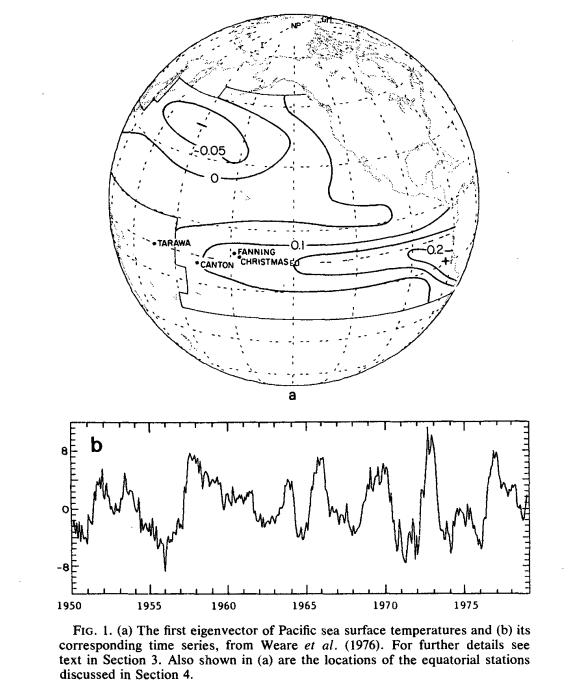
\includegraphics[width=0.4\linewidth]{uploads/Screenshot 2024-11-15 154321.png}
	\caption{Horel and Wallace (1981)}
	\label{fig:1981}
\end{figure}
This prompt was a systematic view with a month timescale variability: they used EOF to analyze 500 mbar data within a month's variability.
\begin{figure}[htp!]
	\centering
	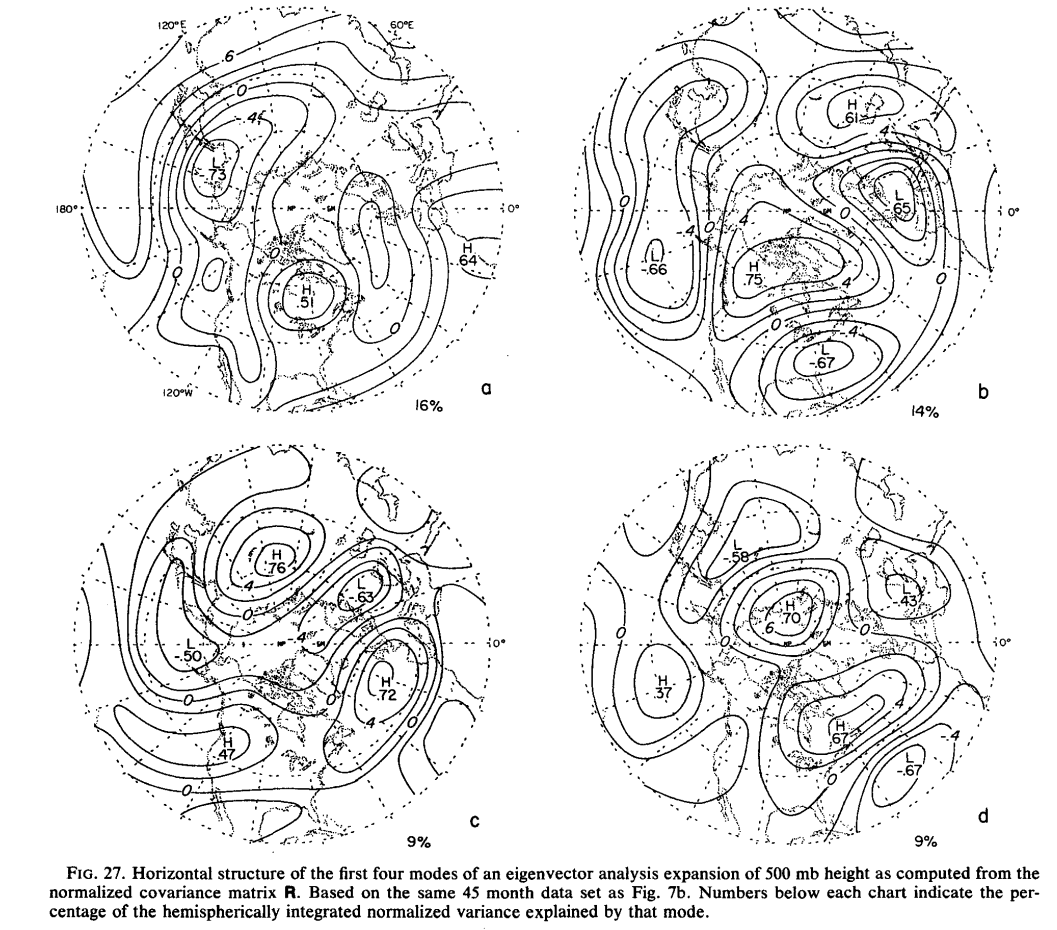
\includegraphics[width=0.45\linewidth]{uploads/Screenshot 2024-11-15 155150.png}
	\caption{Correlation coefficients}
	\label{fig:correlation coeff}
\end{figure}
There are 4 EOFs appearing during the analysis, the matrix had 45 columns (time series). As shown above \ref{fig:correlation coeff}, these patterns are a succession of positive and negative signs. In picture 16\% of variance: reconstructing the timeserie using only that mode, the total variance of that mode will be 16\% of the variance, or, having 45 modes, construct one by change, the change that it will look close to that one is 16\%.

There was a network of connections disappearing beyond the synoptic view.
\begin{figure}[htp!]
	\centering
	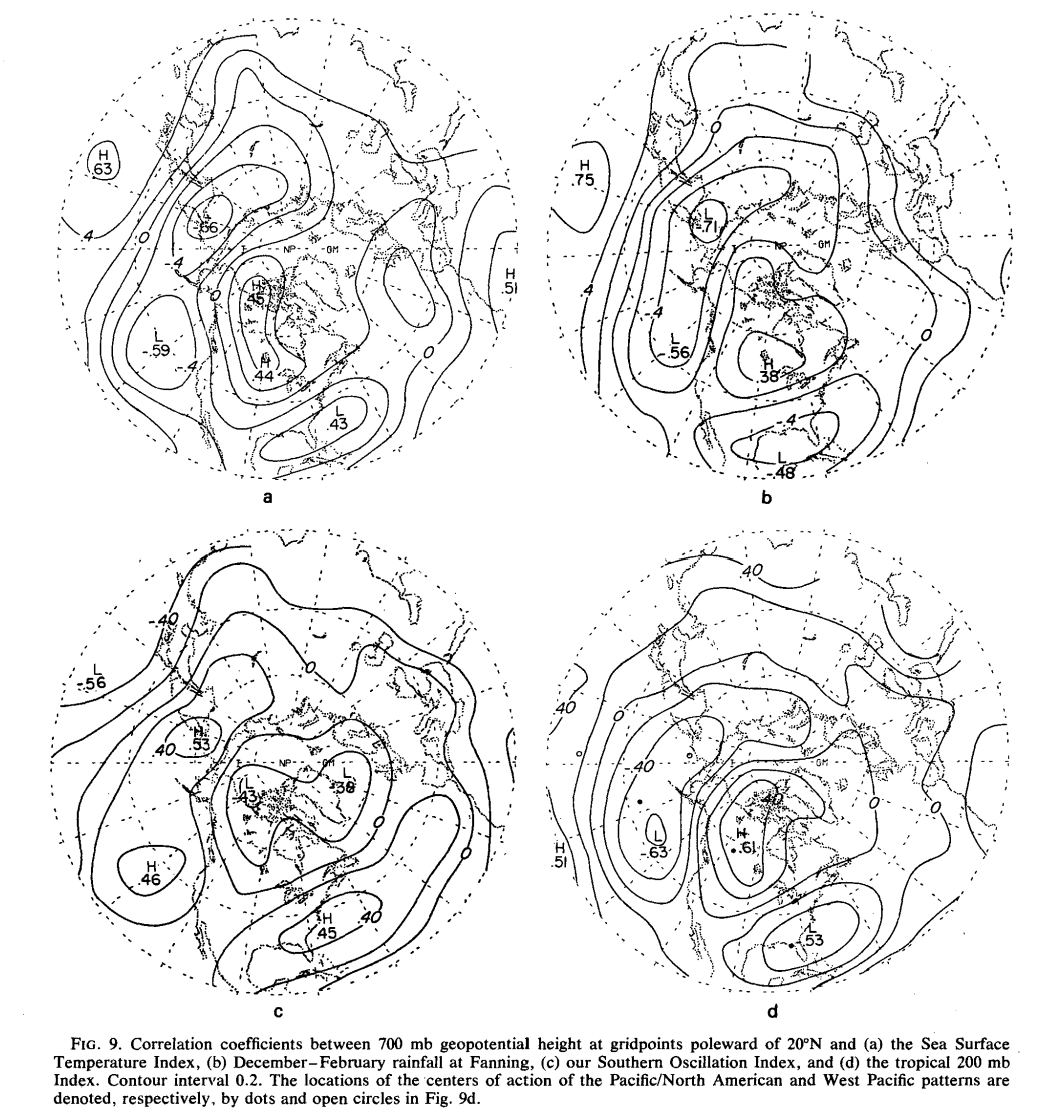
\includegraphics[width=0.4\linewidth]{uploads/imageexploringvar.png}
	\caption{Connected variability in the ocean and in the atmosphere}
	\label{fig:conn var}
\end{figure}


Synoptic variation was understood as an instability of the basic flow. Nonlinear balance is reached if the instability grows very much outside the linear regime, and this could happen in a time series of a week/ten days.
When you try to connect variability in the ocean with the variability in the atmosphere you get a pattern like the figure \ref{fig:conn var}.






The idea came forward that at least a part of this teleconnection must be connected to the Ocean. There's a lot of variability in the ocean at monthly timescales. The figure below \ref{fig:SST VAR} shows deviations from seasonal timescales: a lot of variability at monthly timescales. The figure also shows the strongest El Nino ever recorded in 1993 and in 1998 another El Nino.
\begin{figure}[htpb]
	\centering
	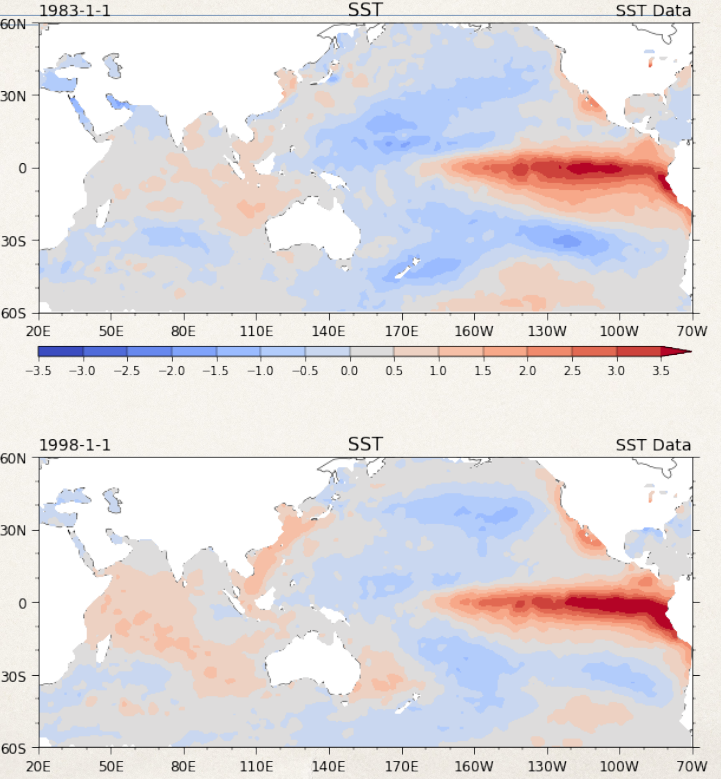
\includegraphics[width=0.35\linewidth]{uploads/Screenshot 2024-11-18 164612.png}\quad 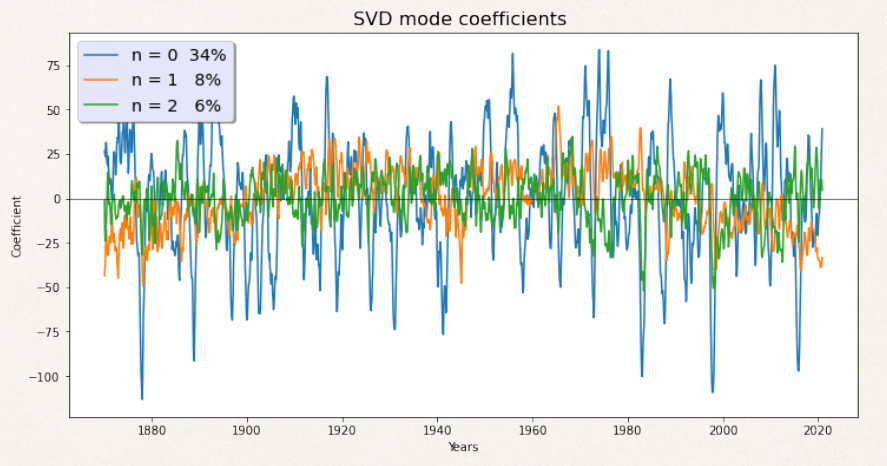
\includegraphics[width=0.5\linewidth]{uploads/Screenshot 2024-11-18 164205.png}
	\caption{SST Variability over a monthly timescale and on the right main EOF timeseries}
	\label{fig:SST VAR}
\end{figure}



The right figure of \ref{fig:SST VAR} represents a modern analysis of SST variability from 1880 to last year. Once the notion that the SST was important became clear, people started to try to record the SST. However, there could have been a problem due to the difference in heat loss between different stations. In the figure, $n=0$ is the first EOF, here you can see huge oscillations (describes ENSO) and the negative phases of ENSO that are oscillating down. From now on started to come out with the idea that there is some periodic behavior.
\begin{figure}[htpb]
	\centering
	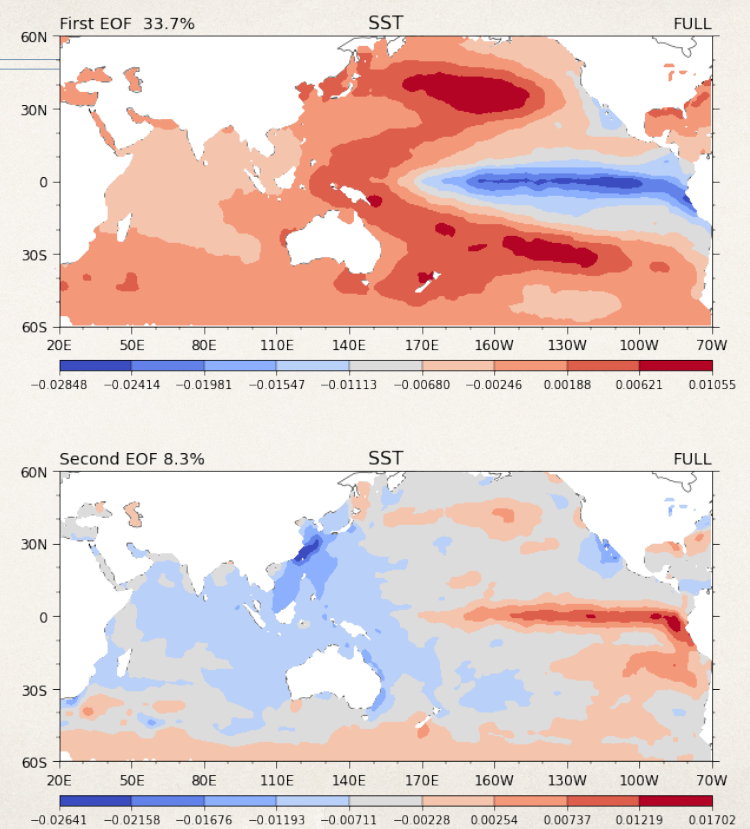
\includegraphics[width=0.35\linewidth]{uploads/Screenshot 2024-11-18 164916.png}
	\caption{First two modes}
	\label{fig:first two modes}
\end{figure}


In figure \ref{fig:first two modes}: the top one of El Nino, EOF cannot separate one phenomenon from the other: there are mathematical constraints (i.e. to be orthogonal to each other). In the following  years, people try to make variations to address some of the problems. EOFs are very sensitive to where the variability is concentrated. As you go to higher modes, you get more structure for two main reasons: modes are getting more complicated and EOFs have to be orthogonal to each other because of their construction. Everything is dominated by the large variations in the equatorial zone, and this variation in the North Pacific is relatively weighted less (here is very uniform but something is going on). Later it was discovered to be the Pacific decayed oscillation.

\section{Designing a model for variability}
All of these evidences were statistics, there is no reason to believe in causation. In order to demonstrate that it is the SST that forms those oscillations, we need to use a climate model and design an experiment.
From evidence of past experiments it is clear that SST is connected to anomaly in the atmosphere, how should we design a model?

We want to design a numerical method, that is a  simulation of climate using the model.
For instance, we would like to see the evolution in time of SST and we have a dataset from 1880.
Considering just the atmosphere, you need initial data in the model and boundary conditions in the ground (topography stressing the presence of mountains, it is not necessary to consider vegetation because it is part of the length scheme of the model, but we need a land-see mask stressing where are lands, oceans and ice). You have to take into account the temperature of the ocean, in this case, SST (integrating forward in time will get a simulation in data). If you want to see the impact of the SST on the atmosphere you change the model inducing a disturbance (for example, changing the boundary conditions at the surface) and you get the monthly mean of SST. This type of experiment is called a \textit{prescribed experiment}.


Run an atmospheric model using prescribed mean SSTs for the entire duration of the simulation. Within this framework, you can introduce an artificial perturbation to the SST in specific regions to observe its effects. For instance, the temperature at 2 meters above the surface (a standard atmospheric variable) is influenced by these SST changes, making it part of the atmospheric problem. By modifying the boundary conditions, such as increasing SSTs in certain areas, the model can reveal the resulting atmospheric responses to these changes.



So they built a strategy to do that: you start with a basic model and you add a perturbation to it. This will lead you to a comparison between one system with the perturbation and the other one without the perturbation, which is called the control system or the reference. Comparing the two systems, you'll gain the effect of the perturbation you applied.

\begin{figure}[htpb]
	\centering
	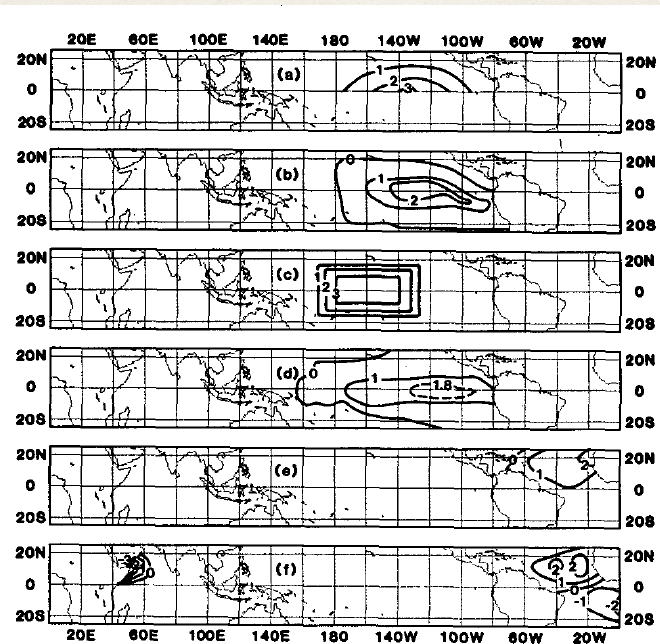
\includegraphics[width=0.35\linewidth]{uploads/Screenshot 2024-11-20 212353.png}
	\caption{the fourth from the top is the paper}

\end{figure}
They did two perturbations and looked at the difference: the model would create a series of anomalies propagating. You create anticyclones in the north and the south of the anomaly. This fact provides an intense investigation of how the monthly scale can predict monthly anomalies. We are taking the difference between two strongly nonlinear simulations, so we are stretching the fact that we can still see the difference.

This means that the relation of the two simulations is quite linear so that the effect of perturbations can be identified. In detail, consider the geopotential at 300 mbar (high atmosphere) \ref{fig:figure 1.7}, it is the streamfunction of the flow.
\begin{figure}[htpb]
	\centering
	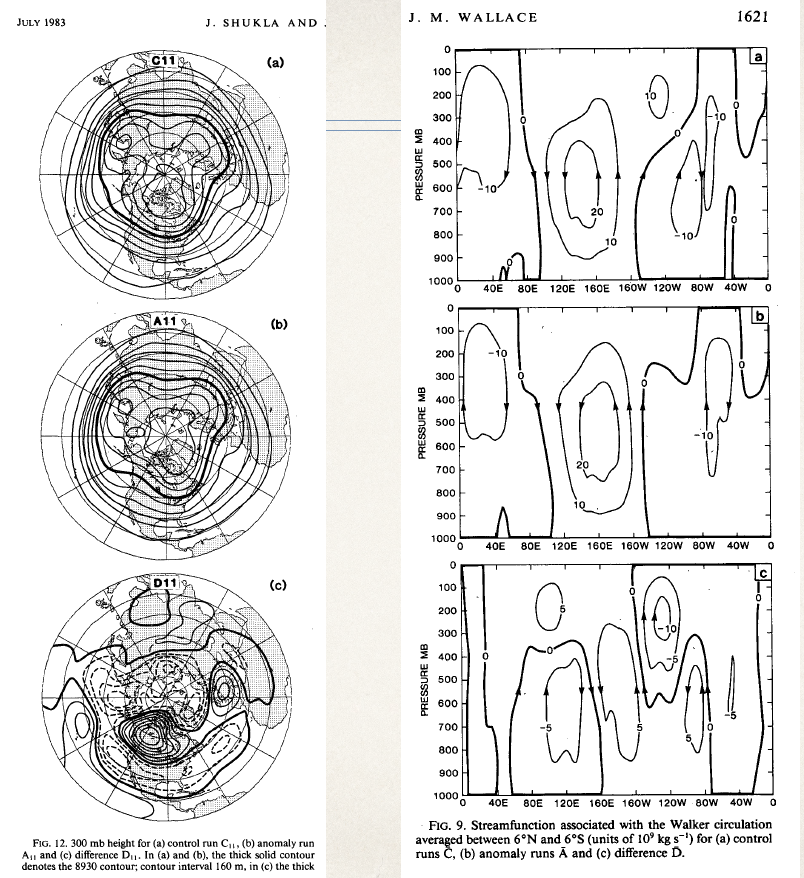
\includegraphics[width=0.4\linewidth]{uploads/Screenshot 2024-11-20 212453.png}
	\caption{A section at the equator between 6N and 6S }
	\label{fig:figure 1.7}
\end{figure}
The one on top is the control simulations, the middle one is the perturbation experiment (with SST in the Pacific) and the bottom one is the difference between the two.
Most of them are concentrated in the North Pacific, related to the SST anomaly in the equatorial Pacific. Note that when you look at the total field the differences are small but still exist.
This was the first evidence that if you have perturbation that will have an impact, that creates a deviation from normal conditions.

Figure \ref{fig:figure 1.7} is a section at the equator between 6N and 6S
the arrows give the sense of circulation; in the difference, you see the extra rising air over the SST (central part or graph). This paper shows that the way SST is acting on the atmosphere is affecting the water circulation, especially increasing the vertical motion over the areas of increased SST. Why exactly air go up?

People decided to set up a special project called AMIP, an Atmospheric Model Intercomparison Project, based on the idea that SST is important but we have many models, expecting the SST in different ways, so how we could compare them?
It was already clear that because of the sensitivity not only of the initial conditions but also to perturbation, it is not enough one simulation.
We know that if we change a little bit initial conditions in any of these models, the evolution is slightly different, and also the response of SST it is; meaning that you have to do different experiments and confront them statistically.

They aren't using idealizing perturbation of the SST but the observed SST month by month. So it was designed a protocol in which all the people participating in the project, could run the models using the same dataset.
\begin{figure}[htp!]
	\centering
	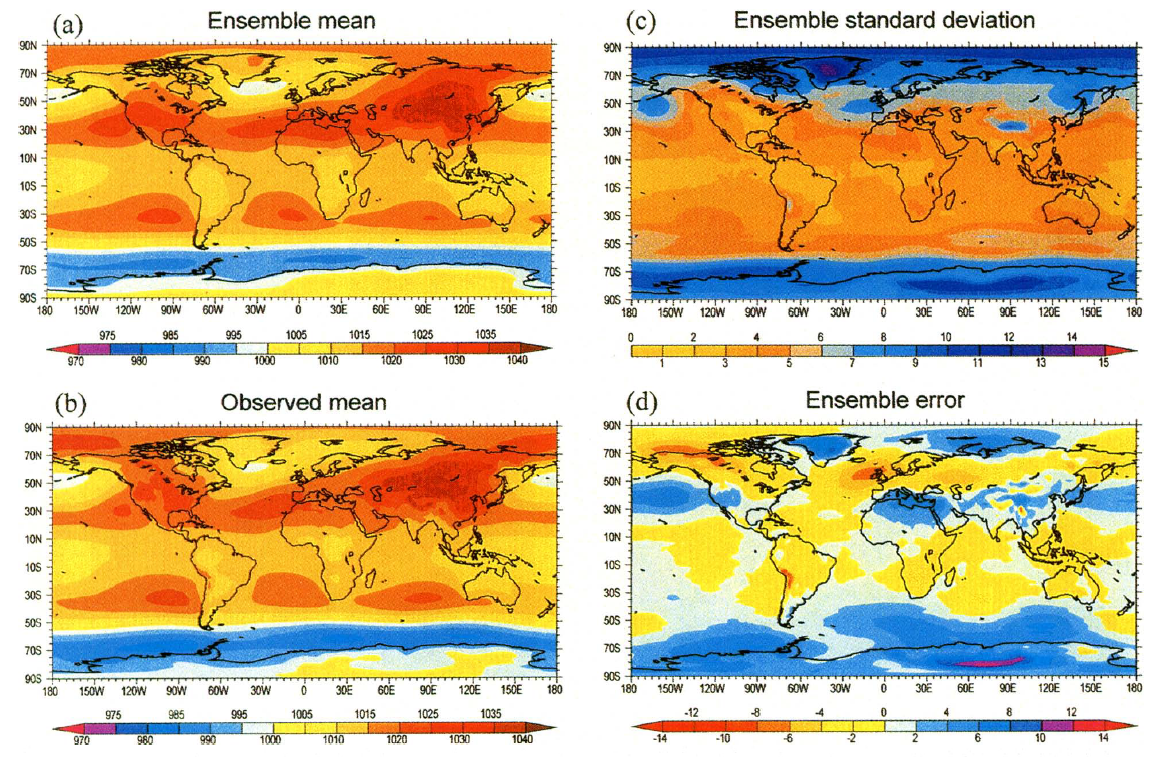
\includegraphics[width=0.45\linewidth]{uploads/Screenshot 2024-11-20 212548.png}\quad 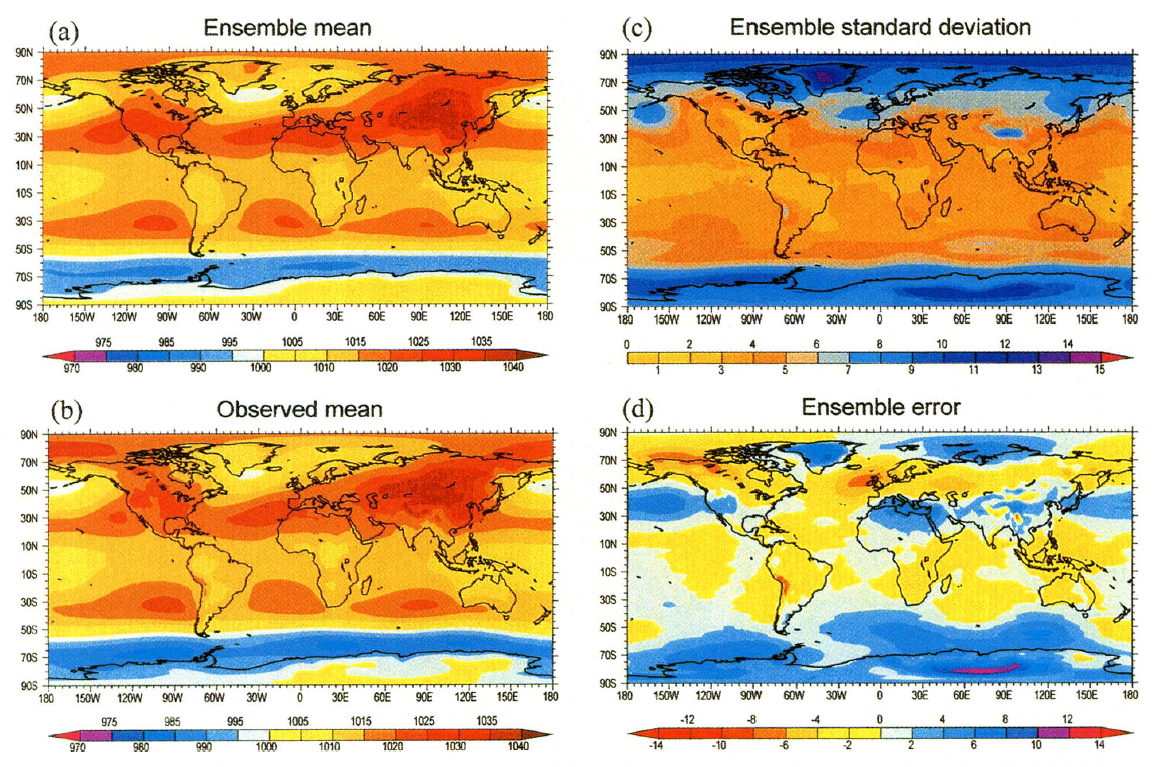
\includegraphics[width=0.45\linewidth]{uploads/Screenshot 2024-11-20 204551.png}
	\caption{a)AMIP results for mean sea level pressure. b)AMIP result for precipitations.}

\end{figure}
As for the mean sea level pressure measured in winter between 1979 and 1988, despite the fact the ensemble means and the observed mean seem to be similar, there is an error of 14 mbar (good or bad depends on what you have to do).
It was clear that there was a systematic problem: models seem to underestimate sea level pressure. If the error had a systematic structure, it could be possible that numerics weren't represented well.
If we look at the standard deviation of the ensemble, we are looking at how these models would agree with each other (most of the deviation is presented in polar regions). In other words, we are looking at the degree of control that SST exerts on the atmosphere. If the control is perfect, all the models will give the same evolution; if not, models have the freedom to do slightly different things.
The SST control is very effective in the tropical regions and in the mid-latitudes (east basin of the ocean). Weaker error occurs over North America, so SST seems capable of controlling the anomaly of circulation over it and the tropics; it seems not to have control over Europe (blob of high standard deviation).

Internal variation (for example, what will happen at 15 o'clock next month) beyond the range of initial conditions cannot be predicted.



The standard deviation is very small over the ocean, meaning the SST is controlling precipitations.
In general, it's much more difficult than the dynamical field, because precipitations are much more difficult than other dynamics since they are driven by physical processes so you need to describe convection and turbulence very well. Other problems are linked with getting the observation and spatial correlation that is difficult. We get good data only recently, especially thanks to satellite like TRIMM that allow us to make estimates of precipitation also over the ocean.


\begin{figure}[htp!]
	\centering
	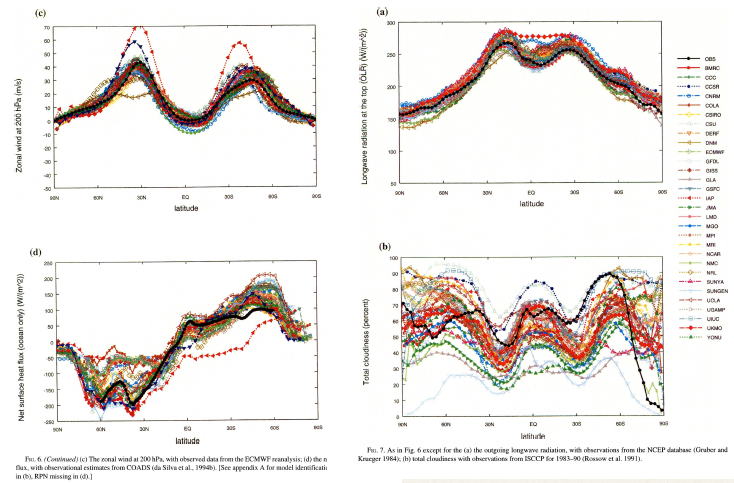
\includegraphics[width=0.6\linewidth]{uploads/Screenshot 2024-11-20 210633.png}
	\caption{all the models participating in the comparison and the observations are the black line}
	\label{fig:9}
\end{figure}
All the models agree on the zonal wind, it means that the dynamics of zonal wind is easy. All the variations you see are how the model is formulated, you start to see differences because different formulation has a big impact, so how people choose to represent them has an impact on the result.
If your balance at the top is not zero the model will cool or warm over 200-300 years

In the figure \ref{fig:9} the panel (b) is a disaster: clouds. That shows clouds are difficult to model.



This kind of result grew in people's determination to insert clouds in models because do not consider them to represent the issue of credibility.


\section{General Circulation Models }
\begin{figure}[htpb]
	\centering
	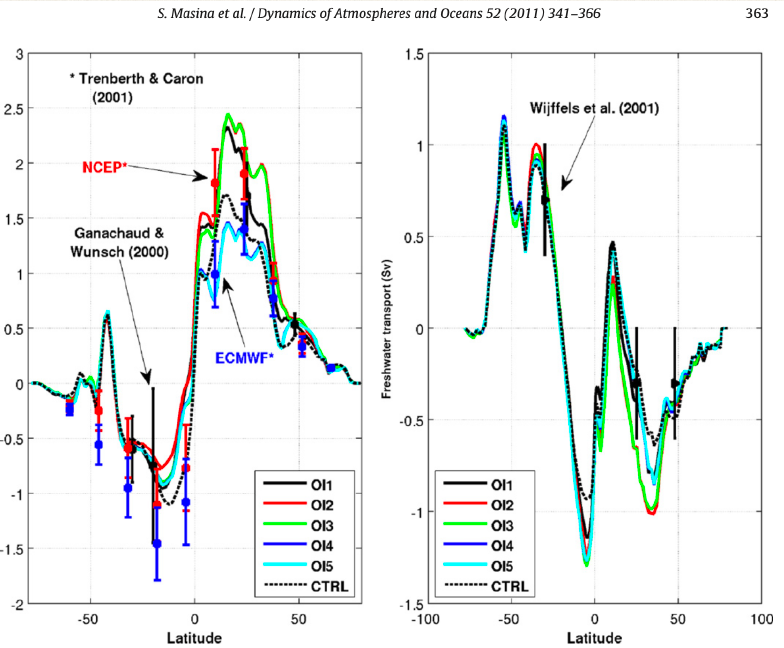
\includegraphics[width=0.4\linewidth]{uploads/image8.png}
	\caption{Climatological global heat transport and fresh-water transport: the different curves are different ocean re-analysis and black lines are observations}

\end{figure}
In the models, there are some variables called prognostic (expressed under time derivative, so they are in the left part of the equation), for atmospheric models, these are temperature, winds and water vapor; while for the ocean models, these are currents, temperature and salinity. Radiation instead, is computed from these variables so it is called a diagnostic variable.
The only way to change temperature and salinity in the ocean is by the interaction between the atmosphere and the ocean.

Independently from which numerical methods, finite differencing or spectral, we use, we need grids.
\begin{figure}[htp!]
	\centering
	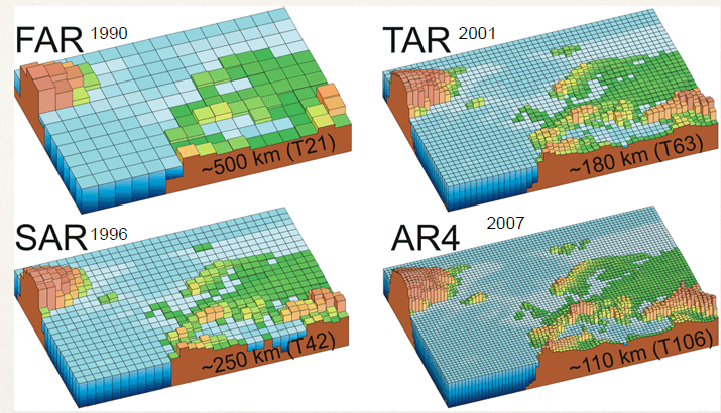
\includegraphics[width=0.4\linewidth]{uploads/Screenshot 2024-11-20 213227.png}
	\caption{Evolution of different models}
	\label{fig:grids evolution}

\end{figure}
As we can see from the picture above \ref{fig:grids evolution}, FAR had a resolution of 500 km for finite differencing and T21 for the spectral method. Now instead we are able to reach a resolution of 30km x 30km and doing that made us capable of starting to detail the oceans.

It takes 5-6 years to collect all the info to have valid results to insert in the Assessment Report, a document that analyzes the state of the art of the science, collecting all the knowledge gained so far.
If you want to do forecasting you want your model to follow exactly the observations. To do that, your initial conditions are important because for the atmospheric models they last 2-3 weeks, while for the oceans they last 12-50 weeks.

Some problems are derived from the observations since they do not cover all over the world uniformly and especially they are concentrated in the continents (which is the best density of station for the observations is still endless discussion, since they are expensive; probably the best thing you can do is to have maximum information with the minimum station distribution).

Really interesting is the ocean observing system which was possible to build thanks to the development in the knowledge of ENSO.
\begin{itemize}
	\item TAO anchorage system to the sea floor in the equator measuring temperature
	\item  ARGO FLOATS float on a systematic depth and every 10 days they change their buoyancy and rise up recording the profile of different variables, after that they go down again
	\item tidal station across the coast of the continents to measure sea level
\end{itemize}

Finally, with all this data collected, you have to fill them in both space and time, creating a physically consistent field of observations around the globe. Since everything you know is in the equations, you will use the models to do the simulations with different techniques developed through the years.


One important thing to take into consideration is that you have to take into account the ocean transport. It plays an important role in the climate system since it restores the imbalance of heat between tropics and polar regions. In particular, there is an excess of radiation energy in the equatorial region and a deficit in the polar region.
\begin{figure}[htpb]
	\centering
	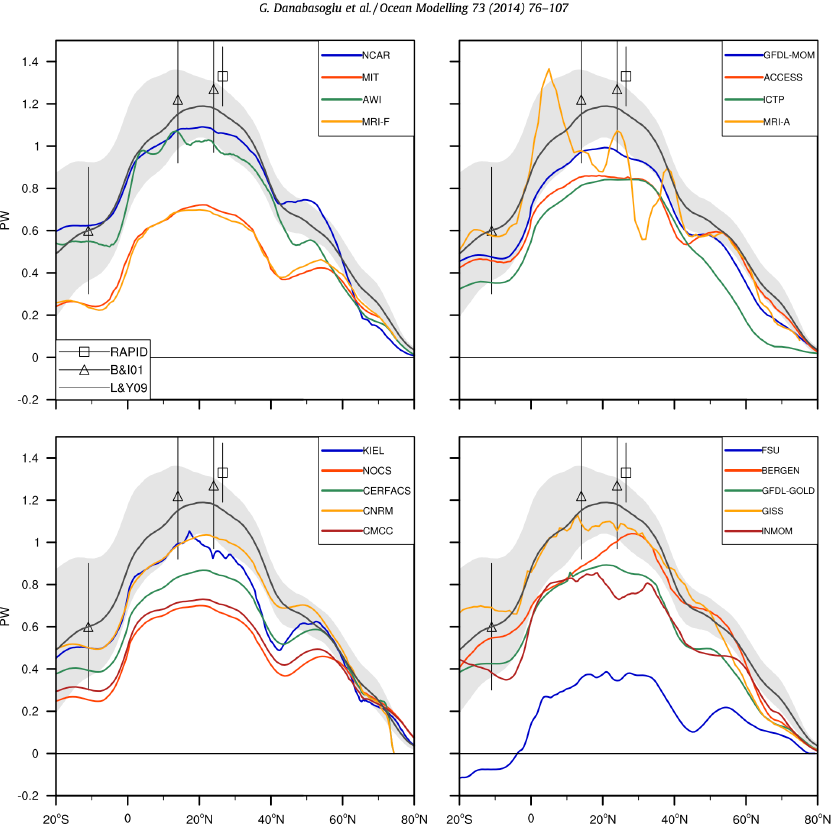
\includegraphics[width=0.5\linewidth]{uploads/image9.png}
	\caption{Time mean meridional heat transports for the Atlantic Ocean with different models}
	\label{fig:12}
\end{figure}
In the picture below \ref{fig:12} the observations are the point and all the lines are model simulations. All the models are underestimating transports.
This graph shows us the main important thing in data assimilation: you have to reduce as better as possible the distance between observations and models. \\






Another important aspect that must be taken into consideration is the AMOC, Atlantic meridional overturning circulation. It is a part of the global circulation of the ocean that starts with the deep water in the North Atlantic where cold waters sink towards the bottom (due to its high salinity that promotes high density).
Controlling the AMOC helps scientists to understand if this process really happens and how effective it is.
If you stop the production of dense water, for example by freshening the North Atlantic with an increase of precipitation, all the AMOC will become weaker.

\begin{figure}[htpb]
	\centering
	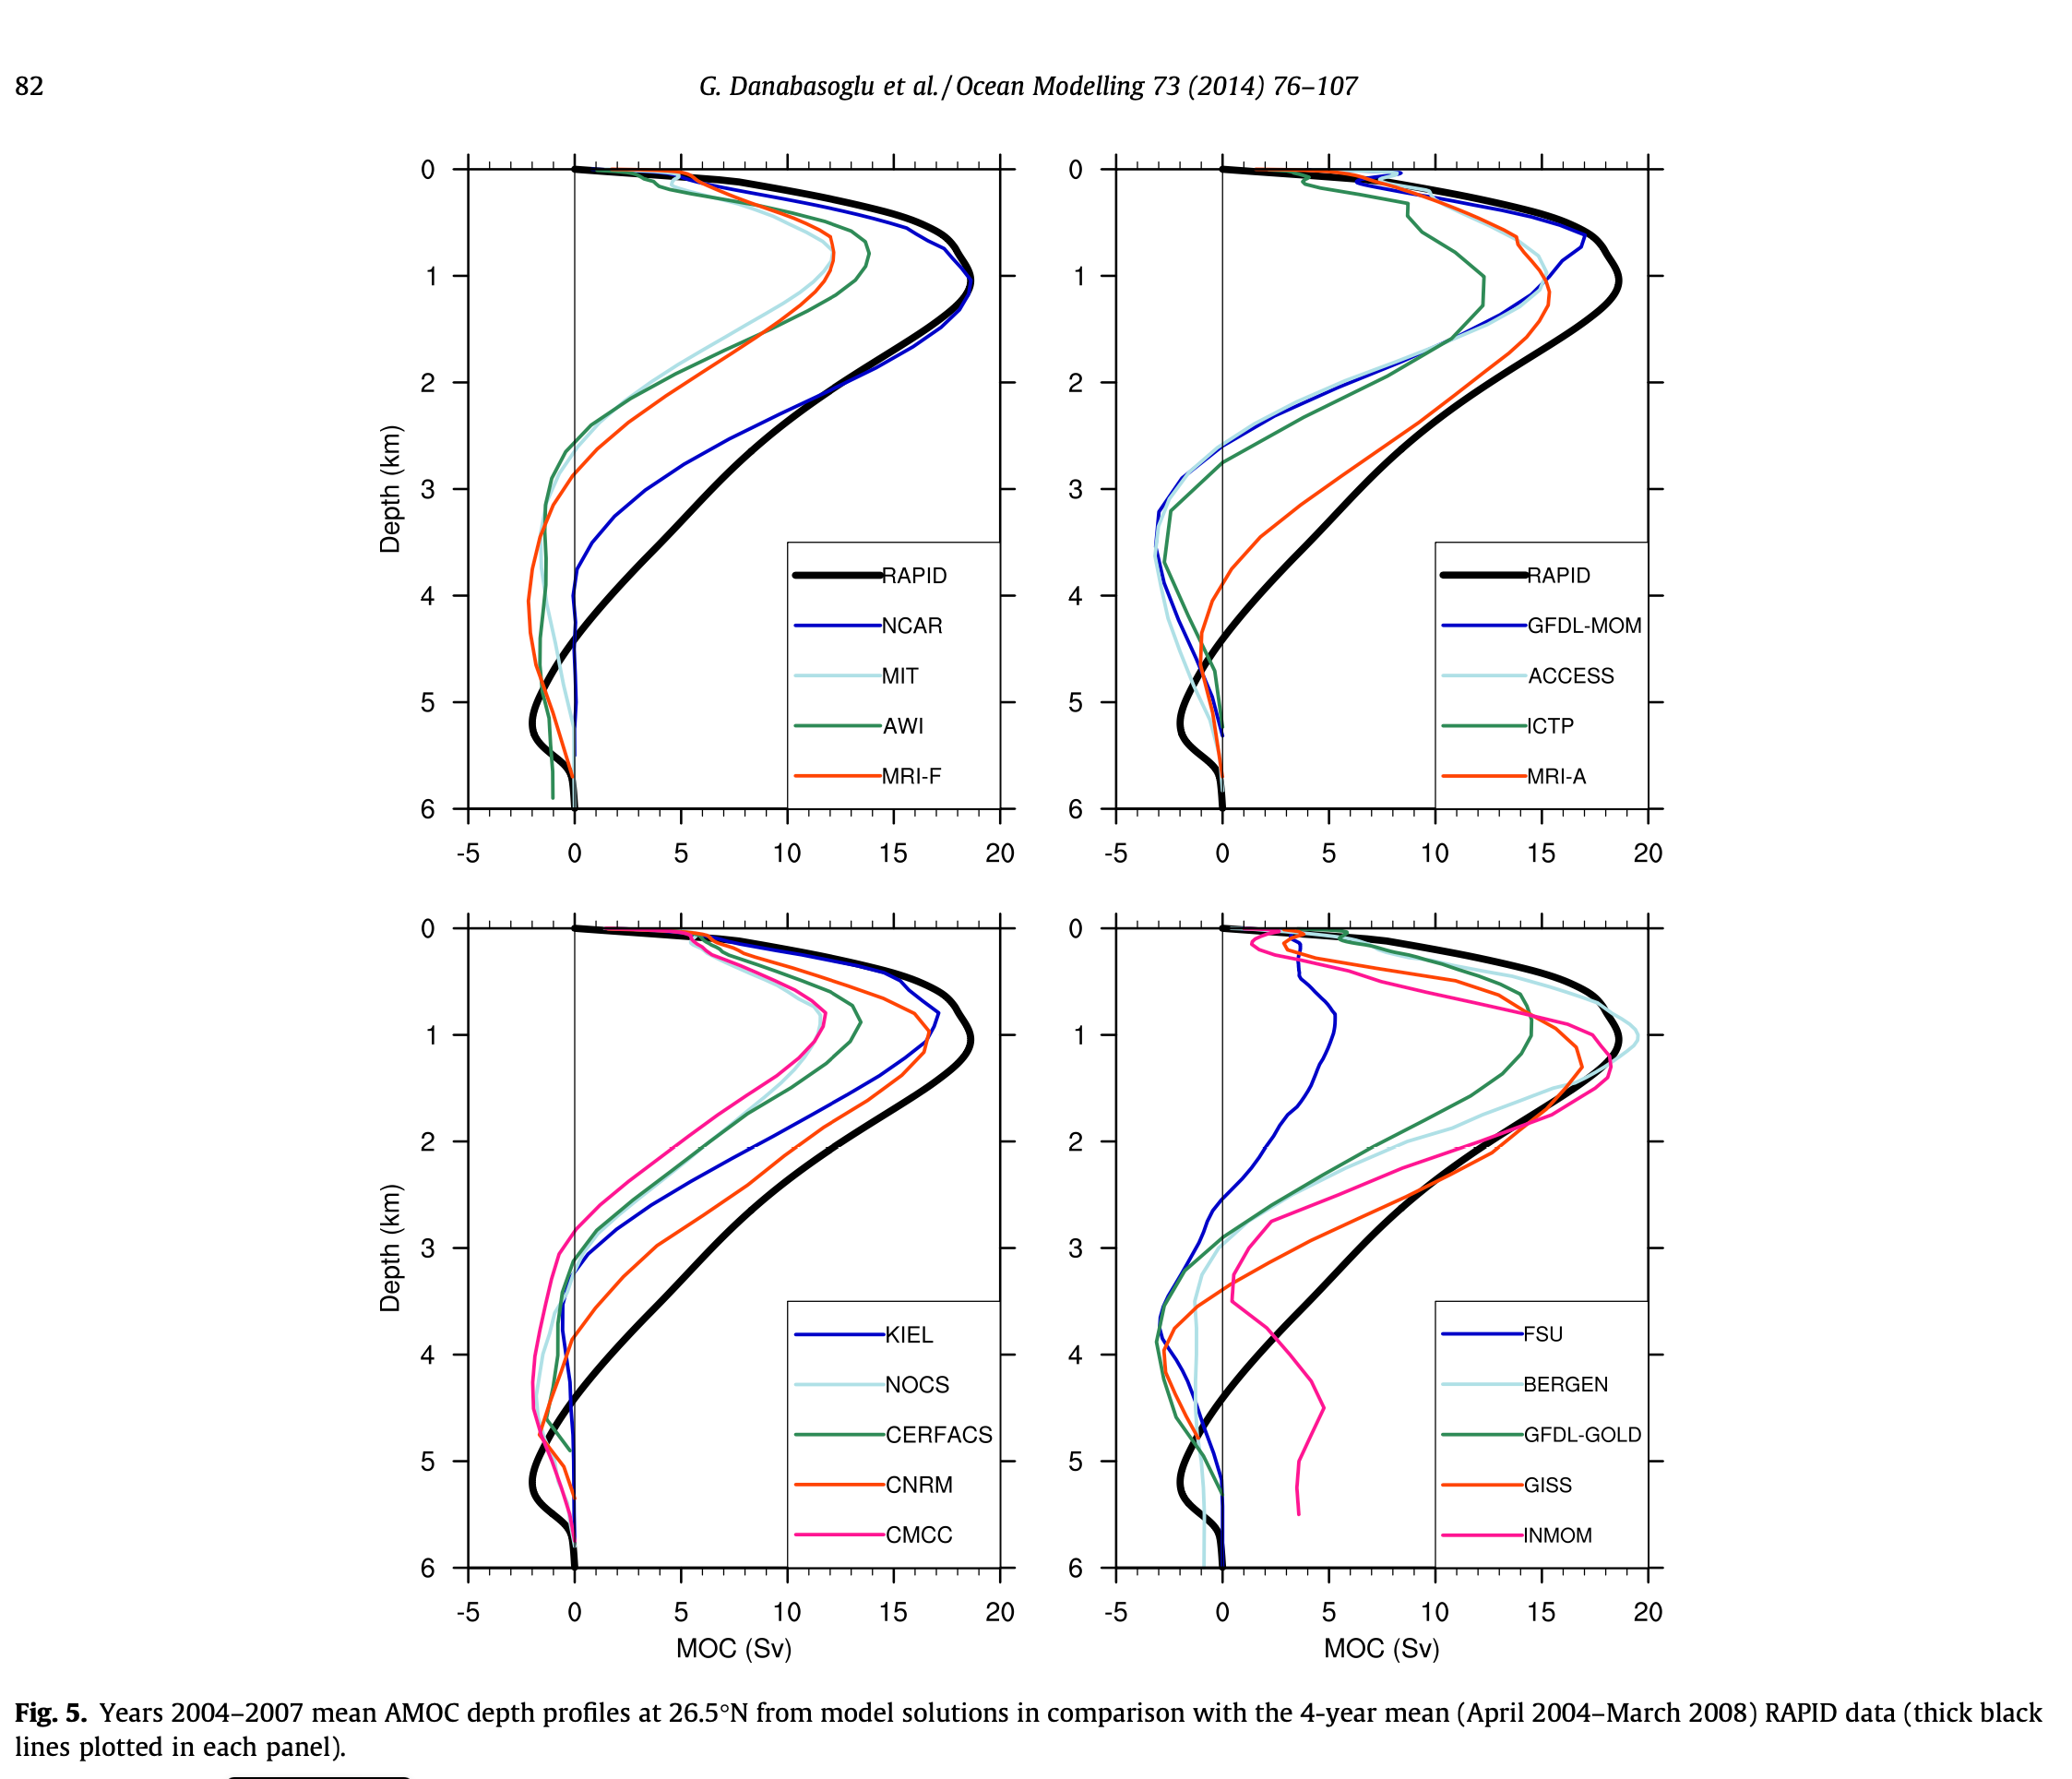
\includegraphics[width=0.6\linewidth]{uploads/image3.png}
	\caption{NCAR doesn't really stress this phenomenon described above, despite the fact it follows observations quite well}

\end{figure}

In recent years, scientists have developed new modes of investigation concerning simulations, experiments, and theories together. Also, improvement of forecasting skills helped them to improve the quality of simulations, specifically in the number of days in which the forecast stopped being useful.
\begin{figure}[htpb]
	\centering
	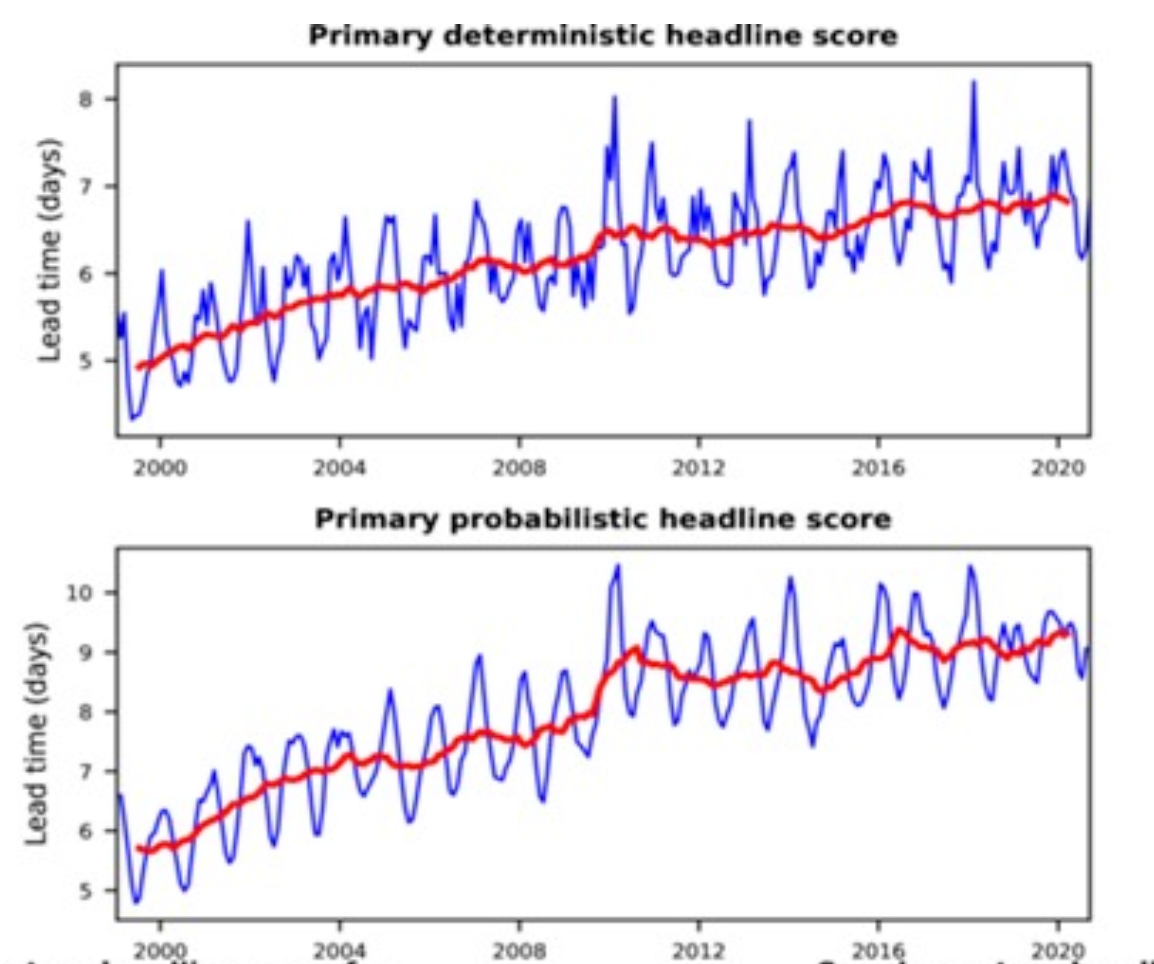
\includegraphics[width=0.5\linewidth]{uploads/image5.png}
	\caption{Improvement in forecasting skills}

\end{figure}

Last but not least, different models have similar patterns of errors. This is a problem because, even if the mean of a variable is correct, I had to consider realistic variability from it. If I improve the initial conditions, I'll improve the short timescale forecast; while if I improve the model, I'll improve the medium timescale forecast.
\begin{figure}[htpb]
	\centering
	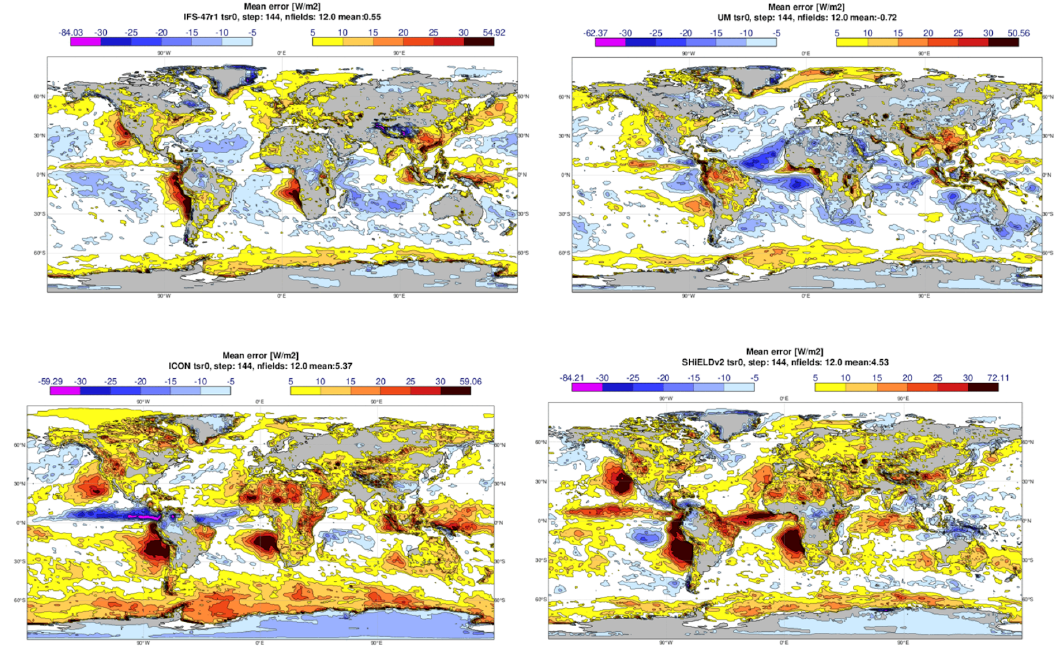
\includegraphics[width=0.7\linewidth]{uploads/image7.png}
	\caption{Example of mean errors in comparison different models}

\end{figure}